\chapter{auto}
\lhead[tempest 2000]{}
\label{sec:bullet}
\lstset{style=68KStyle}

\begin{minipage}[c]{0.48\linewidth}
\begin{figure}[H]
    \centering
    \begin{adjustbox}{width=5cm,center}
      \includegraphics[width=12cm]{src/t2kdemo/demo.png}%
    \end{adjustbox}
\end{figure}
\end{minipage}
\begin{minipage}[c]{0.48\linewidth}
\begin{lstlisting}[basicstyle=\scriptsize\ttfamily]
tst auto      ; Check if in demo-mode.
beq namsg     ; If we're not, skip.
; Draw the demo text.
lea bfont,a1  ; Load the large font
lea autom1,a0 ; "Demo" string
move #50,d0   ; Set y position
jsr centext   ; Display text in center
\end{lstlisting}
\vspace*{\fill}
\end{minipage}

As in the original \textit{Tempest}, managing the attract mode behaviour
of the claw comes down to deciding where to move and when to shoot. What
we find in \textit{Tempest 2000} is that shooting is simplified down to 
'always shoot'. Unlike \textit{Tempest}, no attention is paid to whether
there may be an enemy present or not: the rule is that we will stop and
shoot if there is an enemy on the same lane, and we'll also fire off a
bullet whenever we move left or right. This keeps things simple, but does
mean that we will sit on a lane firing bullets at an enemy until it is
destroyed rather than moving on immediately.

We find this approach compactly implemented at the head of the \icode{claw\_con1}
routine. It outsources the decision on whether left or right movement is the
best choice to a routine called \icode{lor} but looks afer everything else itself.

\begin{lstlisting}
claw_con1:
        move #1,whichclaw    ; Flag that this is player 1. 
        tst auto             ; Are we in demo mode?
        beq sclawr           ; If we're not, use player input. 

        ; Otherwise we're in demo mode, so decide what to do. 
        move.l pad_now,-(a7) ; Stash any player input on the stack.
        move droid_data,d0   ; droid_data has the lane of enemy nearest top.
        bsr lor              ; Decide whether to move left or right.

        bpl moveme           ; If movement selected, perform the movement.
        clr.l 20(a6)         ; Otherwise, stop the claw here.
        move.l fire_1,pad_now ; Press fire.
gscl:   bsr sclawr           ; Shoot a bullet at the enemy.
        move.l (a7)+,pad_now ; Restore stashed player input from the stack.
        rts                  ; We're done - so return.
    
        ; Look after the movement. 
moveme: bne clawright        ; If '0' from 'lor' then move right.
        ; Otherwise We need to move left.
        move.l fire_1,d0     ; Might as well fire a bullet too.
        or.l #$00400000,d0   ; Move left.
        move.l d0,pad_now    ; Add bullet and movement to input.
        bra gscl             ; Move, fire bullet, and return.

clawright:                   ; We need to move right.
        move.l fire_1,d0     ; Might as well fire a bullet too. 
        or.l #$00800000,d0   ; Move right.
        move.l d0,pad_now    ; Add bullet and movement to input.
        bra gscl             ; Move, fire bullet, and return.
\end{lstlisting}

The \icode{lor} subroutine is responsible for figuring out whether the best movement is left or right. On
a plane that is open, i.e. isn't closed like a circle, it's a simple question
of whether the claw is to the right or left of the target and should move
in the opposite direction to get nearer to it. 

\begin{minipage}[c]{0.48\linewidth}
\begin{figure}[H]
    \centering
    \begin{adjustbox}{width=6.5cm,center}
      \includegraphics[width=3cm]{src/t2kdemo/demo_plane_left1.png}%
    \end{adjustbox}
\end{figure}
\end{minipage}
\begin{minipage}[c]{0.06\linewidth}
\begin{figure}[H]
    \centering
    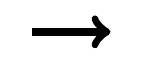
\begin{tikzpicture}[baseline={(current bounding box.south)}]
      \draw[->,line width=3pt] (0,0) to (1,0);
    \end{tikzpicture}
\end{figure}
\end{minipage}
\begin{minipage}[c]{0.48\linewidth}
\begin{figure}[H]
    \centering
    \begin{adjustbox}{width=6.5cm,center}
      \includegraphics[width=3cm]{src/t2kdemo/demo_plane_left2.png}%
    \end{adjustbox}
\end{figure}
\end{minipage}


But in the case of a closed plane, this might be suboptimal. 
So what we do instead is split the closed plane
into two halves. If the target is in a lower-numbered lane than the claw, then
the claw will move left if is in the 'lower' half of the web:

\clearpage
\begin{lstlisting}
; *******************************************************************
; lor: select whether to move left or right
; enter with d0=web column # of target. 
; For any web, returns d1=0 for go left, 1 for go right,
; based on a6 object's position.
; *******************************************************************
lor:    move 16(a6),d1 ; Get the claw's current position.
        cmp d0,d1      ; Compare it to the topmost enemy's.
        bne nntrv      ; If positions not the same, go to nntrv.
        tst auto       ; Are we in demo mode?
        beq nntrv      ; If not, skip to nntrv.
        move #-1,d1    ; Tell demo mode to stop the claw here.
        rts            ; Return.

        ; Where position of claw and target are not the same, figure
        ; out whether to go left or right.
nntrv:  tst connect    ; Is it a closed/wrapper web?
        bne _lor1      ; If so, skip to _lor1 to handle it..
        ; (1) Othwerise the web is a plane that doesn't wrap so subtracting
        ; positions will tell us which way to move.
        sub d0,d1      ; Subtract the position of target from the claw. 
        bgt lor0       ; If greater than 0, move left..
        ble lor1       ; If less than 0, move right..

        ; (2) Otherwise the web is a 'closed plane' that wraps, so need to
        ; figure the shortest path to the enemy.
_lor1:  move web_max,d2; Get number of lanes in web and put it in d2.
        asr #1,d2      ; Divide by 2 to get half total lanes in web.
        sub d0,d1      ; Subtract the position of target from the claw. 
        bgt _lll       ; If target in a lower lane than claw, go to _lll.  
        ble _rrr       ; If target in a higher lane than claw, go to _rrr.  
        ; With target in a lower lane than the claw, if the claw is in 
        ; the 'lower' half of the web then it should move left, otherwise
        ; it should move right.
_lll:   sub d2,d1      ; Subtract halfway-point in web from claw position.
        blt lor0       ; If it's less than zero, move left..
        bra lor1       ; Otherwise move right.

        ; With target in a higher lane than the claw, if the claw is in 
        ; the 'lower' half of the web then it should move right, otherwise
        ; it should move left.
_rrr:   neg d1       
        sub d2,d1      ; Subtract halfway-point in web from claw position.
        blt lor1       ; If it's less than zero, move right..
                       ; .. otherwise move left.
lor0:   clr d1         ; Decided to move left, so set d1 to 0.
        rts            ; Return
lor1:   move #1,d1     ; Decided to move right, so set d1 to 1.
        rts            ; Return
\end{lstlisting}
\clearpage

\begin{minipage}[c]{0.48\linewidth}
\begin{figure}[H]
    \centering
    \begin{adjustbox}{width=6.5cm,center}
      \includegraphics[width=3cm]{src/t2kdemo/demo_left1.png}%
    \end{adjustbox}
\end{figure}
\end{minipage}
\begin{minipage}[c]{0.06\linewidth}
\begin{figure}[H]
    \centering
    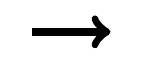
\begin{tikzpicture}[baseline={(current bounding box.south)}]
      \draw[->,line width=3pt] (0,0) to (1,0);
    \end{tikzpicture}
\end{figure}
\end{minipage}
\begin{minipage}[c]{0.48\linewidth}
\begin{figure}[H]
    \centering
    \begin{adjustbox}{width=6.5cm,center}
      \includegraphics[width=3cm]{src/t2kdemo/demo_left2.png}%
    \end{adjustbox}
\end{figure}
\end{minipage}

Otherwise it will move right:

\begin{minipage}[c]{0.48\linewidth}
\begin{figure}[H]
    \centering
    \begin{adjustbox}{width=6.5cm,center}
      \includegraphics[width=3cm]{src/t2kdemo/demo_left1.png}%
    \end{adjustbox}
\end{figure}
\end{minipage}
\begin{minipage}[c]{0.06\linewidth}
\begin{figure}[H]
    \centering
    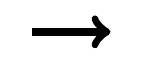
\begin{tikzpicture}[baseline={(current bounding box.south)}]
      \draw[->,line width=3pt] (0,0) to (1,0);
    \end{tikzpicture}
\end{figure}
\end{minipage}
\begin{minipage}[c]{0.48\linewidth}
\begin{figure}[H]
    \centering
    \begin{adjustbox}{width=6.5cm,center}
      \includegraphics[width=3cm]{src/t2kdemo/demo_left3.png}%
    \end{adjustbox}
\end{figure}
\end{minipage}

Likewise if the target is in a higher-numbered lane than the claw,
then the claw will move right if it is in the 'lower' half of the web:

\begin{minipage}[c]{0.48\linewidth}
\begin{figure}[H]
    \centering
    \begin{adjustbox}{width=6.5cm,center}
      \includegraphics[width=3cm]{src/t2kdemo/demo_left1.png}%
    \end{adjustbox}
\end{figure}
\end{minipage}
\begin{minipage}[c]{0.06\linewidth}
\begin{figure}[H]
    \centering
    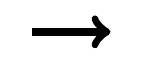
\begin{tikzpicture}[baseline={(current bounding box.south)}]
      \draw[->,line width=3pt] (0,0) to (1,0);
    \end{tikzpicture}
\end{figure}
\end{minipage}
\begin{minipage}[c]{0.48\linewidth}
\begin{figure}[H]
    \centering
    \begin{adjustbox}{width=6.5cm,center}
      \includegraphics[width=3cm]{src/t2kdemo/demo_left3.png}%
    \end{adjustbox}
\end{figure}
\end{minipage}

Otherwise it will move left:

\begin{minipage}[c]{0.48\linewidth}
\begin{figure}[H]
    \centering
    \begin{adjustbox}{width=6.5cm,center}
      \includegraphics[width=3cm]{src/t2kdemo/demo_left1.png}%
    \end{adjustbox}
\end{figure}
\end{minipage}
\begin{minipage}[c]{0.06\linewidth}
\begin{figure}[H]
    \centering
    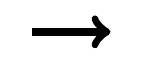
\begin{tikzpicture}[baseline={(current bounding box.south)}]
      \draw[->,line width=3pt] (0,0) to (1,0);
    \end{tikzpicture}
\end{figure}
\end{minipage}
\begin{minipage}[c]{0.48\linewidth}
\begin{figure}[H]
    \centering
    \begin{adjustbox}{width=6.5cm,center}
      \includegraphics[width=3cm]{src/t2kdemo/demo_left3.png}%
    \end{adjustbox}
\end{figure}
\end{minipage}

